\documentclass[10pt]{article}
\usepackage[letterpaper,margin=1in]{geometry}
\usepackage[T1]{fontenc}
\usepackage{mathptmx}
\usepackage[scaled=0.92]{helvet}
\usepackage{courier}
\usepackage{microtype}
\usepackage{amsmath,amssymb,amsthm}
\usepackage{graphicx}
\usepackage{booktabs}
\usepackage{multirow}
\usepackage{enumitem}
\usepackage{xcolor}
\usepackage[numbers,sort&compress]{natbib}
\usepackage{algorithm}
\usepackage{algpseudocode}
\usepackage[colorlinks=true,linkcolor=blue!50!black,citecolor=blue!50!black,urlcolor=blue!50!black]{hyperref}
\usepackage[capitalise,noabbrev]{cleveref}
\usepackage{caption}
\captionsetup{font=small,labelfont=bf}

\newtheorem{proposition}{Proposition}
\newtheorem{corollary}{Corollary}
\theoremstyle{definition}
\newtheorem{definition}{Definition}
\crefname{proposition}{Proposition}{Propositions}
\crefname{corollary}{Corollary}{Corollaries}

\newcommand{\skc}{\textsc{SKC}}

\title{\textbf{Keep the Ledger, Drop the Logs:\\State-Keyed Context Compaction for Long-Horizon LLM Agents}}
\author{Anonymous Authors}
\date{}

\begin{document}
\maketitle

\begin{abstract}
Long-horizon LLM agents must compress their growing interaction histories, and
most compressors treat the history as text to be shortened---by recency,
masking, salience or summarization. We argue that an agent's history is better
viewed as an \emph{event log that mutates a state}, and that what compression
must preserve is the \emph{current value of each state variable}. This view
exposes two failure modes: \emph{missing} state, and the more insidious
\emph{stale} state, where the newest value is dropped but an older one survives.
We formalize compression with keyed state writes and an ideal reader and prove
that the compacted log (the latest record per key) is a sufficient statistic
whose size is independent of the horizon; that supersession-consistent
compressors are never stale while recency windows forget keys by age; and that
supersession-blind selection is stale with probability
$(1-\rho)(1-(1-\rho)^{m-1})$ for a key with $m$ writes, a law that also governs
imperfect extraction. We propose State-Keyed Compaction (SKC), a model-free
compressor with three layers: a verbatim latest-value ledger, supersession-aware
deduplication, and a knapsack scored by a utility model trained for free from
logged trajectories. Across 4{,}979 public trajectories from two agent scaffolds
and twelve LLM configurations, 65--89\% of context tokens are tool outputs and
23--55\% are repeated lines. On 2{,}479 held-out trajectories, SKC keeps
7--9 points more state than the best of seven baselines in-domain
(e.g.\ 65.0\% vs.\ 57.8\% at a $4.7\times$ compression) and 3--6 points more on
unseen scaffolds and LLMs, with stale rates (0.1--0.3\%) as low as a recency
window. With three LLM readers from two families, SKC raises the accuracy of
questions about the agent's current state from 25--40\% to 50--77\%
($p<10^{-3}$) without degrading next-action prediction, while LLM summaries
answer only 2--7\%. Fine-grained lexical selection still preserves more of the
code that agents re-type; an oracle utility shows that this gap is one of
prediction, which our framework can absorb.
\end{abstract}

%% ---------------------------------------------------------------------------
\section{Introduction}
\label{sec:intro}

Large language model (LLM) agents now routinely run for tens to hundreds of
steps: a software-engineering agent opens files, edits them, runs tests, reads
tracebacks, and edits again~\citep{yang2024sweagent,wang2025openhands}. Every
step appends an action and an observation to the context, and tool outputs
dominate it: in the 1{,}478 SWE-agent trajectories we study, \textbf{71--89\% of
all context tokens are tool outputs} (\cref{sec:corpus}). Even when a model's
window is large enough, long contexts cost latency and money and degrade
accuracy~\citep{liu2024lost,hsieh2024ruler,hong2025contextrot}. Every practical
agent therefore \emph{compresses} its history---by truncating it, masking old
observations, pruning ``unimportant'' tokens, or summarizing it with an
LLM~\citep{packer2023memgpt,lindenbauer2025complexity,kang2025acon,anthropic2025context}.

Most of these methods treat the history as \emph{text to be shortened}. We argue
that for agents it is better viewed as an \emph{event log that mutates a state}.
An edit changes a region of a file; re-running a test replaces the previous
result; a user's correction overrides an earlier constraint. What the agent
must not lose is the \emph{current value of each state variable}, and a
compressor can fail in two distinct ways: it can drop the value
(\emph{missing}), or---worse---drop the latest value while keeping an older one,
so that a capable reader confidently acts on an outdated state
(\emph{stale}). Text-centric criteria such as recency or relevance do not see
this distinction: a relevance scorer has no reason to prefer the newer of two
test results, and a recency window has no reason to keep a constraint stated
fifty steps ago.

This view suggests borrowing a mechanism that databases have used for decades:
\emph{log compaction}, which retains only the latest record per
key~\citep{kreps2011kafka,kleppmann2017ddia}. We make the idea precise and test
it.

\paragraph{Contributions.}
\begin{enumerate}[leftmargin=*,itemsep=1pt,topsep=2pt]
  \item \textbf{A state-centric formalization} of agent context compression
  (\cref{sec:formulation}): histories as event logs with keyed writes, an
  \emph{ideal reader} that separates information loss from reader ability, and
  three outcomes---\emph{correct}, \emph{stale}, \emph{missing}---for each
  state probe.
  \item \textbf{Theory} (\cref{sec:theory}): the compacted log is a sufficient
  statistic whose size is independent of the horizon and matches an
  information-theoretic lower bound; \emph{supersession-consistent} compressors
  (which include recency windows and the compacted log) can never be stale;
  recency windows lose keys at a rate governed by key age rather than
  importance; and any compressor that keeps turns independently of supersession
  incurs a stale rate of $(1-\rho)(1-(1-\rho)^{m-1})$ for a key with $m$ writes
  when it keeps a fraction $\rho$ of turns---which also describes a ledger fed by
  an extractor with recall $\rho$.
  \item \textbf{State-Keyed Compaction (SKC)} (\cref{sec:method}): a simple,
  model-free compressor that keeps a latest-value-per-key ledger with verbatim
  values and provenance, a short raw window, and a skeleton of older actions,
  allocating the budget with a knapsack-ratio priority; and a hybrid,
  SKC+BM25, that the theory shows can add relevance-based selection without
  creating stale state.
  \item \textbf{An empirical study} on 1{,}478 real SWE-agent trajectories from
  five LLMs (GPT-4, Claude~3 Opus, GPT-4o, Claude~3.7 Sonnet, Claude~4 Sonnet)
  and on a controllable benchmark, \textsc{StateTrack}
  (\cref{sec:setup,sec:results}). We measure, for six compressors and budgets
  of 4k--16k tokens, how much agent state survives compression, how often a
  compressor leaves only stale state, and how well it preserves information
  that the agent actually goes on to use.
\end{enumerate}

\paragraph{Scope.} This paper measures \emph{information sufficiency}: whether
the compressed context still contains what an ideal reader would need. It does
not run LLM agents end-to-end on compressed contexts. Sufficiency is a
necessary condition for downstream success and isolates the compressor from
the reader; the price is that our numbers are upper bounds on what a real model
can recover (\cref{sec:limitations}). All code, parsed probes and results are
released.

%% ---------------------------------------------------------------------------
\section{Related Work}
\label{sec:related}

\paragraph{Prompt and context compression.} Token-level pruning methods drop
tokens with low self-information or low importance under a small LM, e.g.\
Selective Context~\citep{li2023selective} and the LLMLingua
family~\citep{jiang2023llmlingua,jiang2024longllmlingua,pan2024llmlingua2}.
Learned compressors map context into soft tokens~\citep{mu2023gist,chevalier2023autocompressors,ge2024icae},
and KV-cache methods evict entries by attention statistics or position~\citep{zhang2023h2o,xiao2024streamingllm}.
These methods score text by salience; they are not designed around
supersession, which our analysis shows is what produces stale state. Our BM25
baseline~\citep{robertson2009bm25} is a turn-level, model-free representative of
salience-based selection.

\paragraph{Memory for LLM agents.} MemGPT pages information between a bounded
context and external storage~\citep{packer2023memgpt}; Generative Agents keep a
memory stream with recency/importance/relevance retrieval and periodic
reflection~\citep{park2023generative}; Reflexion stores verbal
lessons~\citep{shinn2023reflexion}. MemoryBank, A-MEM and Mem0 organize long-term
memories, and Mem0 explicitly applies add/update/delete operations to stored
facts~\citep{zhong2024memorybank,xu2025amem,chhikara2025mem0}. Recursive or
gist summarization compresses long documents and
dialogues~\citep{wang2023recursively,lee2024readagent,chen2023memwalker}.
Benchmarks such as LoCoMo and LongMemEval test long-term conversational memory
including knowledge updates~\citep{maharana2024locomo,wu2025longmemeval}. Our
work is complementary: rather than proposing another memory architecture, we
give a formal account of \emph{what} must be preserved within a single
long-horizon episode, why common compressors fail, and an evaluation that
separates missing from stale state.

\paragraph{Context management for long-horizon agents.} Closest to us,
\citet{lindenbauer2025complexity} show that simply masking old observations in
SWE-agent matches LLM summarization in solve rate at lower cost, and
ACON~\citep{kang2025acon} optimizes compression guidelines for history and
observations with failure-driven feedback. MEM1 trains agents to maintain a
compact internal state that replaces the history~\citep{zhou2025mem1}.
Practitioner guidance recommends ``compaction'' and structured note-taking for
agents~\citep{anthropic2025context}. We provide the missing analytical lens:
observation masking works because agent turns carry most state-changing
information and because it is (nearly) supersession-consistent; it fails on
state that only lives in observations. SKC can be seen as making the implicit
state of these approaches explicit and keyed.

\paragraph{State tracking and logs.} Language models' ability to track entity
states through a sequence of operations is studied by
\citet{kim2023entity}. Event sourcing and log compaction in data systems keep
only the latest record per key so that the state can be rebuilt from a bounded
log~\citep{kreps2011kafka,kleppmann2017ddia}; streaming lower
bounds~\citep{alon1999space} motivate our counting argument.

%% ---------------------------------------------------------------------------
\section{Problem Formulation}
\label{sec:formulation}

\paragraph{Histories and state.} An agent history is a sequence of turns
$h_{1:t}=(x_1,\dots,x_t)$, each a piece of text of $\ell(x_i)$ tokens with a
role (task, agent, tool, user). Let $\mathcal{K}$ be a set of \emph{state keys}
and $\mathcal{V}$ a set of values. Each turn carries a (possibly empty) set of
\emph{writes} $\mathrm{W}(x_i)\subseteq\mathcal{K}\times\mathcal{V}$: evidence
that key $k$ took value $v$ at time $i$. The state at time $t$ is the
\emph{fold} of the log under last-writer-wins,
\begin{equation}
  S_t(k) = v \quad\text{where } (k,v)\in \mathrm{W}(x_i),\; i=\max\{j\le t: k \text{ written in } x_j\},
\end{equation}
and $S_t(k)=\bot$ if $k$ was never written. For a software agent, keys include
the content of each edited file region, the latest output of each command, the
latest view of each file window, the results of each code search, and the task
itself (\cref{sec:setup}).

\paragraph{Compressors.} A compressor $C$ maps a history and a budget $B$ to a
context $c=C(h_{1:t},B)$: a sequence of \emph{units}, each either a (possibly
truncated or masked) turn or a derived record, with total length at most $B$
tokens (a fixed system prompt is kept and not charged).

\paragraph{Ideal reader and outcomes.} To separate what a compressor removes
from what a particular LLM can exploit, we evaluate with an \emph{ideal reader}
$R^\ast$ that, for a key $k$, finds in $c$ the evidence of the most recent write
to $k$ that is still present. Writes carry \emph{evidence}: a set of normalized
lines that identify the value (\cref{sec:setup}); a write is present if some
unit contains at least a fraction $\theta=0.8$ of its evidence lines. A
\emph{state probe} $(k,t)$ then has one of three outcomes:
\begin{itemize}[leftmargin=*,itemsep=1pt,topsep=2pt]
  \item \textbf{correct}: the latest write to $k$ is present;
  \item \textbf{stale}: the latest write is absent but an older write with a
  different value is present---a capable reader would act on outdated state;
  \item \textbf{missing}: no write to $k$ is present.
\end{itemize}
We report, for each compressor and budget, the fraction of probes in each class.
Stale outcomes are strictly worse than missing ones: a missing value can be
re-acquired (e.g.\ by re-running a command) if the agent notices the gap,
whereas a stale value gives no signal that anything is wrong.

\paragraph{Use probes.} State probes require a definition of keys, which could
favor a method built on the same keys. We therefore also use a key-free,
behavior-grounded measure: at each decision point we take the identifiers
(names, dotted names, paths; \cref{app:probes}) in the agent's \emph{next
action} that already occurred earlier in the history but not in the system
prompt, and ask whether each is still \emph{available} somewhere in the
compressed context. This measures whether compression removes information the
agent actually went on to use.

%% ---------------------------------------------------------------------------
\section{Theory}
\label{sec:theory}

Proofs are in \cref{app:proofs}. Write $\mathrm{L}_t$ for the \emph{compacted
log}: for every key written up to time $t$, the record of its latest write.

\begin{proposition}[Sufficiency and size of the compacted log]
\label{prop:sufficiency}
For every key $k$, $R^\ast(\mathrm{L}_t,k)=S_t(k)$. Its size
$|\mathrm{L}_t| = \sum_{k\in\mathcal{K}_t}|\mathrm{rec}(k)|$ depends only on the
set $\mathcal{K}_t$ of keys written so far and on their current values, not on
the number of turns or on the number of writes.
Conversely, any compressor whose context lets $R^\ast$ answer every probe
correctly, for all histories over $K$ keys with values in $\mathcal{V}$, must use
contexts of at least $K\log_2|\mathcal{V}|$ bits for some history.
\end{proposition}

Thus the compacted log is optimal up to the encoding of keys and values, and the
cost of a full-retention memory grows with the number of \emph{live keys}, not
with the horizon. Long agent runs are long mostly because the same keys are
rewritten (tests re-run, files re-viewed); compaction removes exactly this
redundancy.

\begin{definition}[Supersession consistency]
A compressor is \emph{supersession-consistent} (SC) if, for every key, the set
of its writes present in the context is a suffix of its write sequence: whenever
a write to $k$ is present, every later write to $k$ is present too.
\end{definition}

\begin{proposition}[SC compressors are never stale]
\label{prop:sc}
If $C$ is SC, every probe outcome is correct or missing. A recency window that
keeps whole turns is SC; so is the compacted log with a perfect extractor; and
so is any union of SC contexts.
\end{proposition}

\begin{proposition}[Recency windows forget by age, not importance]
\label{prop:window}
A recency window of $W$ tokens answers a probe on $k$ correctly iff the latest
write to $k$ lies within the last $W$ tokens. If tool steps have i.i.d.\ lengths
with mean $\mu$ and $k$ is written as a Poisson process with rate $\lambda_k$
per step, then, approximating the token distance by $\mu$ times the age in steps, the
stationary probability that $k$ is retained is $1-e^{-\lambda_k W/\mu}$.
\end{proposition}

Keys that are written rarely---the task statement, a constraint, the location
of the bug found early on---are exactly the ones a window drops first, however
important they are. Masking observations raises the effective $W$ for keys
written in agent turns (edits) but not for keys that live in tool outputs.

\begin{proposition}[Stale rate of supersession-blind selection]
\label{prop:stale}
Let a compressor keep each turn independently with probability $\rho$
(independently of which writes it carries). For a key with $m$ writes in
distinct turns,
\begin{equation}
\Pr[\text{correct}]=\rho,\qquad
\Pr[\text{stale}]=(1-\rho)\bigl(1-(1-\rho)^{m-1}\bigr),\qquad
\Pr[\text{missing}]=(1-\rho)^m .
\label{eq:stale}
\end{equation}
Hence the stale rate increases monotonically in $m$ towards $1-\rho$, and among
probes for which \emph{some} value is present, the fraction that is stale tends
to $1-\rho$ as $m\to\infty$.
\end{proposition}

Two consequences matter in practice. First, salience scores (BM25, token
importance, attention) do not depend on supersession, so selection methods
approach \cref{eq:stale}: under tight budgets, \emph{most} of the values they
retain for frequently updated keys are outdated. Second, the same formula
governs a ledger fed by an imperfect extractor: if each write is detected
independently with recall $r$, the ledger behaves like independent selection
with $\rho=r$ and stops being SC. Extraction errors therefore surface as stale
state, not merely as missing state---the motivation for keeping a raw recent
window next to the ledger (\cref{sec:method}).

\begin{corollary}[A ledger makes selection safe]
\label{cor:safe}
Let $c=\mathrm{L}'\cup c'$, where $\mathrm{L}'\subseteq\mathrm{L}_t$ is any subset
of the compacted log and $c'$ is \emph{any} other context (e.g.\ turns chosen by
relevance). A probe on $k$ can be stale only if $k$'s record is not in
$\mathrm{L}'$. In particular, with the full compacted log, every probe is
correct regardless of $c'$.
\end{corollary}

The corollary licenses a hybrid: once the latest value of each key is pinned in
the ledger, the remaining budget can be spent on supersession-blind but
otherwise useful selection (e.g.\ relevance to the current step) without
creating stale state.

\begin{proposition}[Budgeted ledgers]
\label{prop:knapsack}
If the compacted log exceeds the budget and key $k$ is probed with probability
$p_k$, maximizing the expected number of correct probes is a 0/1 knapsack with
values $p_k$ and weights $|\mathrm{rec}(k)|$. Greedy selection by
$p_k/|\mathrm{rec}(k)|$ is optimal for the fractional relaxation and, combined
with the best single record, a $\tfrac12$-approximation~\citep{dantzig1957knapsack}.
\end{proposition}

%% ---------------------------------------------------------------------------
\section{State-Keyed Compaction}
\label{sec:method}

SKC instantiates the analysis with four parts (\cref{alg:skc}).

\paragraph{Extraction.} An extractor maps each turn to writes. For tool-using
agents most writes are \emph{structural}: they follow from the tool call
itself, which the framework already has in parsed form. For SWE-agent we derive
keys deterministically from actions: \texttt{edit:<file>\#<region>} for the text
written by an edit (regions are tracked so that only edits to overlapping lines
or to text produced by an earlier edit supersede each other),
\texttt{view:<file>@<window>} for file content shown to the agent,
\texttt{search:<query>} and \texttt{cmd:<command>} for the outputs of searches
and (normalized) shell commands. Free-text writes (e.g.\ a user revising a
constraint) require a learned or rule-based extractor; we model its errors by
its recall $r$.

\paragraph{Ledger.} For every key, SKC keeps only the latest extracted write,
rendered \emph{verbatim} (values are capped at $V$ tokens, keeping head and
tail), with provenance (\texttt{[state] key (as of turn i)}). Verbatim values
avoid the paraphrase drift of LLM summaries; provenance lets the reader order
records.

\paragraph{Budget allocation.} The task statement is pinned and the last $R$
turns are kept verbatim. Ledger records whose source turn is already in the
window are skipped. Remaining records are admitted greedily by the knapsack
ratio of \cref{prop:knapsack}, with probe probability estimated as
$p_k = w_{\mathrm{type}(k)}\cdot \tau/(\tau+\mathrm{age}_k)$, where the type
prior favors edits over command outputs, searches and views
($w=4,2,1.5,1$) and $\tau=20$ steps.

\paragraph{Skeleton.} Any budget left is spent extending the raw window
backwards with whole turns and, once a tool output no longer fits, with agent
turns only (older tool outputs replaced by a placeholder), as in observation
masking. We call this variant \textbf{SKC}. A second variant,
\textbf{SKC+BM25}, spends the leftover budget on the older turns with the highest
BM25 score against the task and the latest agent turn, which
\cref{cor:safe} makes safe with respect to staleness.

\begin{algorithm}[t]
\caption{State-Keyed Compaction (SKC)}
\label{alg:skc}
\small
\begin{algorithmic}[1]
\Require history $x_{1:t}$ (task $x_1$), budget $B$, extractor $E$, recent turns $R$, value cap $V$
\State $c \gets [x_1]$; \quad $c_{\text{recent}} \gets$ last $R$ turns (truncate the last turn if it alone exceeds the budget)
\State $\mathrm{L} \gets \{\}$; \textbf{for} $i=2..t$, \textbf{for} $(k,v)\in E(x_i)$: $\mathrm{L}[k]\gets(v,i)$ \Comment{log compaction}
\State $\mathcal{C}\gets\{\textsc{Record}(k,\textsc{Cap}(v,V),i) : (k,(v,i))\in \mathrm{L},\ x_i\notin c_{\text{recent}}\}$
\State sort $\mathcal{C}$ by $p_k/|\textsc{Record}_k|$ descending; admit records while the budget allows
\State \textbf{SKC}: extend backwards from $x_{t-R}$ with whole turns while they fit, then agent turns only (tool outputs masked)
\State \textbf{SKC+BM25}: instead, add older turns by BM25 score against (task, latest agent turn) while they fit
\State \Return $c \,\Vert\, \text{ledger records (by provenance)} \,\Vert\, \text{skeleton} \,\Vert\, c_{\text{recent}}$
\end{algorithmic}
\end{algorithm}

SKC needs no model calls: extraction is a parse of the tool call, compaction is
a dictionary update, and allocation is a sort. It is therefore cheap enough to
run before every step, and it is idempotent: recompressing a compressed history
does not compound errors, unlike recursive summarization.

%% ---------------------------------------------------------------------------
\section{Experimental Setup}
\label{sec:setup}

\paragraph{Real trajectories.} We use the public SWE-agent trajectories submitted
to the SWE-bench Lite leaderboard~\citep{jimenez2024swebench,yang2024sweagent}
by five LLMs spanning two interface generations: GPT-4, Claude~3 Opus and GPT-4o
with the SWE-agent 0.x interface, and Claude~3.7 Sonnet and Claude~4 Sonnet with
SWE-agent 1.x (1{,}478 trajectories in total; \cref{tab:corpus}). Each
trajectory is parsed into a system turn, the task (issue text), and alternating
agent and tool turns; state writes are derived from actions as described in
\cref{sec:method} and \cref{app:probes}. For each trajectory and budget
$B\in\{4\text{k},8\text{k},16\text{k}\}$ tokens we evaluate up to six decision
points whose uncompressed history exceeds $B$ (7{,}949 / 6{,}227 / 4{,}572
decision points), probing every key written so far (125k / 119k / 114k state
probes per compressor) and every eligible identifier in the next action (40k /
37k / 31k use probes).

\paragraph{\textsc{StateTrack}.} The synthetic benchmark generates agent-like
trajectories with three key families: \emph{pinned} constraints stated in the
task and occasionally revised by the user ($p=0.004$ per key and step),
\emph{slow} facts rewritten rarely ($p=0.03$), and \emph{fast} status variables
rewritten often ($p=0.25$). Writes appear as \texttt{key = value} lines inside
tool outputs (80\%) or agent notes (20\%), surrounded by log-like distractor
lines (lognormal, mean 25 lines per output). Values are unique, so the ideal
reader is exact. Unless stated otherwise we use 150 steps, 4 pinned, 12 slow and
6 fast keys, 30 seeds, and probe all keys at three checkpoints.

\paragraph{Compressors.} We compare SKC and SKC+BM25 with five model-free
baselines covering the main families used in practice (settings in
\cref{app:settings}): \textbf{recency window} (FIFO truncation with the task
pinned), \textbf{observation masking}~\citep{lindenbauer2025complexity},
\textbf{truncate observations} (cap each older tool output), \textbf{BM25
selection} (salience-based selection, a turn-level stand-in for
importance-pruning methods~\citep{li2023selective,jiang2023llmlingua}), and
\textbf{random selection}. We do not include LLM summarization, which
requires running an LLM over every prefix; see \cref{sec:limitations}.

\begin{table}[t]
\centering
\small
\caption{SWE-agent trajectories used in this study (SWE-bench Lite). Tokens are
counted over task, agent and tool turns of the full trajectory. ``Far
$>$10'': fraction of identifiers used in an action that first appeared more than
10 steps earlier.}
\label{tab:corpus}
\begin{tabular}{lrrrrrrr}
\toprule
Model (interface) & Traj. & \multicolumn{2}{c}{Steps} & \multicolumn{2}{c}{Tokens} & Tool & Far \\
 & & median & p90 & median & p90 & share & $>$10 \\
\midrule
GPT-4 (0.x)            & 300 & 20 & 34 & 13.1k & 24.7k & 79\% & 33\% \\
Claude 3 Opus (0.x)    & 300 & 18 & 23 &  7.9k & 11.8k & 82\% & 21\% \\
GPT-4o (0.x)           & 278 & 40 & 65 & 22.6k & 49.5k & 89\% & 67\% \\
Claude 3.7 Sonnet (1.x)& 300 & 29 & 54 & 27.3k & 51.6k & 81\% & 61\% \\
Claude 4 Sonnet (1.x)  & 300 & 59 & 91 & 34.7k & 56.7k & 71\% & 79\% \\
\bottomrule
\end{tabular}
\end{table}

%% ---------------------------------------------------------------------------
\section{Results}
\label{sec:results}

\subsection{What long agent contexts are made of}
\label{sec:corpus}

\Cref{tab:corpus} and \cref{fig:corpus} characterize the trajectories. Tool
outputs make up 71--89\% of all tokens. Newer models run longer and reach
further back: for Claude~4 Sonnet the median trajectory has 59 steps and 35k
tokens, and 79\% of the identifiers its actions use first appeared more than
ten steps earlier (21\% for Claude~3 Opus). State writes split into command
outputs (35\%), file views (33\%), edits (27\%) and searches (5\%); a median
trajectory rewrites 4--7 keys at least once. Long horizons therefore come with
both long-range dependencies and frequent overwrites---exactly the two
conditions under which our analysis predicts that windows lose state and
selection produces stale state.

\begin{figure}[t]
\centering
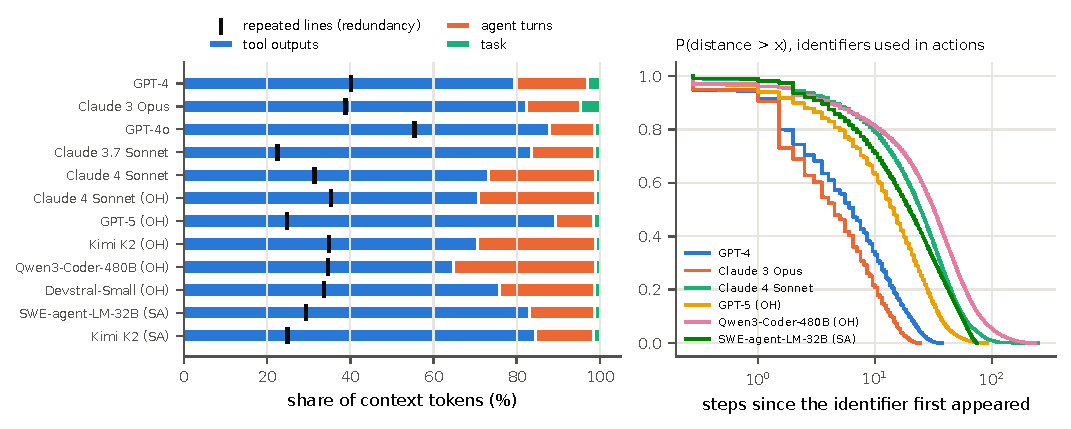
\includegraphics[width=\linewidth]{figures/corpus.pdf}
\caption{Left: share of context tokens by turn type. Right: survival function of
the distance (in steps) between an identifier's first occurrence and its use in
an action.}
\label{fig:corpus}
\end{figure}

\subsection{Main results on real trajectories}
\label{sec:main}

\begin{table}[t]
\centering
\small
\caption{Real SWE-agent trajectories, pooled over five models. State probes: \%
correct and \% stale (the rest are missing). Use probes: \% of identifiers used
by the next action that are still available; ``long'': those last seen more
than two steps earlier. Best in \textbf{bold}.}
\label{tab:main}
\setlength{\tabcolsep}{4pt}
\begin{tabular}{l rrr rrr rrr}
\toprule
 & \multicolumn{3}{c}{State correct $\uparrow$} & \multicolumn{3}{c}{State stale $\downarrow$} & \multicolumn{3}{c}{Use (long) available $\uparrow$} \\
\cmidrule(lr){2-4}\cmidrule(lr){5-7}\cmidrule(lr){8-10}
Compressor & 4k & 8k & 16k & 4k & 8k & 16k & 4k & 8k & 16k \\
\midrule
Recency window        & 40.0 & 52.0 & 66.1 & 0.3 & 0.2 & \textbf{0.1} & 63.0 & 82.9 & 92.8 \\
Observation masking   & 38.8 & 43.1 & 39.0 & 0.3 & 0.3 & 0.6 & 63.3 & 81.5 & 88.7 \\
Truncate observations & 43.1 & 52.5 & 62.1 & 0.6 & 1.0 & 1.3 & 70.3 & 84.5 & 90.2 \\
BM25 selection        & 39.4 & 46.8 & 58.3 & 1.6 & 1.7 & 1.7 & \textbf{76.4} & \textbf{89.9} & 95.2 \\
Random selection      & 51.8 & 63.6 & 75.5 & 2.4 & 1.9 & 1.2 & 71.4 & 84.7 & 93.6 \\
\midrule
SKC (ours)            & \textbf{66.2} & 76.4 & 83.0 & \textbf{0.1} & \textbf{0.1} & \textbf{0.1} & 71.1 & 83.4 & 93.1 \\
SKC+BM25 (ours)       & 66.1 & \textbf{76.7} & \textbf{83.1} & 0.4 & 0.3 & 0.3 & 72.2 & 88.2 & \textbf{95.6} \\
\bottomrule
\end{tabular}
\end{table}

\begin{figure}[t]
\centering
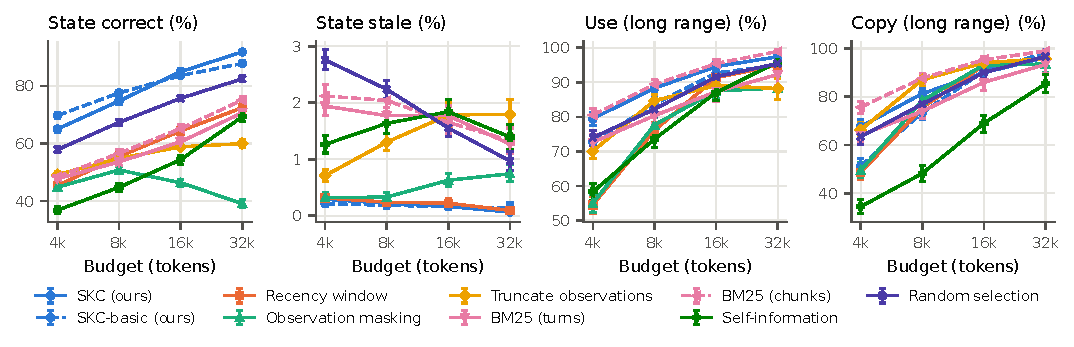
\includegraphics[width=\linewidth]{figures/real_budget.pdf}
\caption{Real trajectories, pooled over five models, as a function of the budget.}
\label{fig:real-budget}
\end{figure}

\paragraph{State retention.} \Cref{tab:main} and \cref{fig:real-budget}
summarize the main comparison. At every budget SKC retains far more of the
agent's state than any baseline: 66\% / 76\% / 83\% of state probes are
correct at 4k / 8k / 16k tokens, versus 40\% / 52\% / 66\% for the recency
window and 39\% / 43\% / 39\% for observation masking. The gain holds for each
of the five models (\cref{tab:by-model} in the appendix): at 8k, SKC improves
over the best non-random baseline by 12 (Claude~3 Opus) to 27 (Claude~4
Sonnet) points, and is within 2 points of or above every baseline for every
model. Random selection is the strongest baseline on this metric because it
spreads the budget over the whole history, but it pays for it in staleness
(below).

\paragraph{Staleness.} Supersession-blind selection leaves stale state:
BM25 and random selection are stale on 1.2--2.4\% of all probes, 12--24 times
more than SKC (0.1\%). The aggregate hides the dependence on overwrites
predicted by \cref{prop:stale}: among keys written three or more times, 9--11\%
of BM25 and random probes are stale, i.e.\ 10--16\% of the values these
methods retain for such keys are outdated (\cref{fig:stale-real}). Recency
windows and observation masking, which are (nearly) supersession-consistent,
stay at or below 2.3\% even for frequently rewritten keys; residual staleness comes
from truncated turns and from edits whose evidence is only partially kept.

\begin{figure}[t]
\centering
\begin{minipage}{0.37\linewidth}
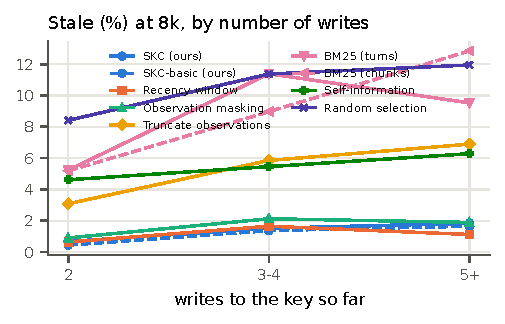
\includegraphics[width=\linewidth]{figures/real_stale_nwrites.pdf}
\end{minipage}\hfill
\begin{minipage}{0.6\linewidth}
\caption{Stale rate on real trajectories (8k) by the number of writes the key
has received. Selection methods (BM25, random) approach the regime predicted by
\cref{prop:stale}; supersession-consistent methods stay low. Keys written once
cannot be stale.}
\label{fig:stale-real}
\end{minipage}
\end{figure}

\paragraph{Forgetting by age.} \Cref{fig:real-age} (left) breaks state probes
down by the age of the key's latest write. Recency windows and observation
masking are as good as SKC for keys written in the last five steps and
collapse beyond ten: for keys last written 21--40 steps ago, 14\% (window) and
10\% (masking) are retained, versus 70\% for SKC, which degrades gracefully
(58\% beyond 40 steps). This is \cref{prop:window} in action: windows forget by
age, regardless of importance.

\begin{figure}[t]
\centering
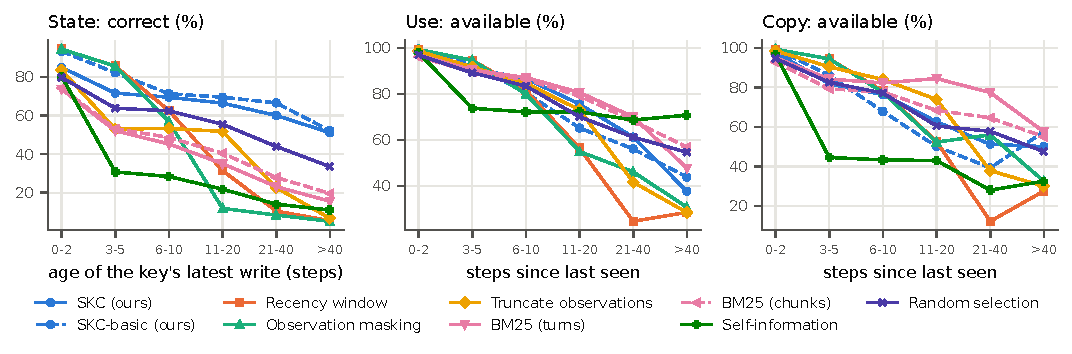
\includegraphics[width=\linewidth]{figures/real_age.pdf}
\caption{Real trajectories at 8k. Left: state probes by the age of the key's
latest write. Right: use probes by the number of steps since the identifier
last appeared.}
\label{fig:real-age}
\end{figure}

\paragraph{Per key family.} \Cref{tab:by-family} shows where the gains come
from. SKC retains 87\% of command outputs and 92\% of search results at 8k
(window: 50\% and 41\%), because these are small, high-value records once the
long outputs around them are dropped. Edits improve from 50--57\% to 75\%. File
views are the exception: they are large (often a 100-line window), have the
lowest priority, and are cut by the value cap, so SKC retains 52\% of them,
below random selection (64\%). This is a deliberate trade-off of the default
priority, analysed further in the ablations.

\begin{table}[t]
\centering
\small
\caption{Real trajectories at 8k: \% correct by key family (and \% stale for
the mutable families). The task is pinned by every method. Probe counts: edit
24.5k, view 32.0k, cmd 47.9k, search 8.5k, task 6.2k.}
\label{tab:by-family}
\setlength{\tabcolsep}{4pt}
\begin{tabular}{l rrrrr rrrr}
\toprule
 & \multicolumn{5}{c}{Correct (\%)} & \multicolumn{4}{c}{Stale (\%)} \\
\cmidrule(lr){2-6}\cmidrule(lr){7-10}
Compressor & task & edit & view & cmd & search & edit & view & cmd & search \\
\midrule
Recency window        & 100 & 50.2 & 49.3 & 50.3 & 40.9 & 0.6 & 0.2 & 0.1 & 0.0 \\
Observation masking   & 100 & 51.6 & 38.9 & 35.7 & 33.7 & 0.9 & 0.5 & 0.1 & 0.0 \\
Truncate observations & 100 & 56.7 & 28.9 & 56.9 & 69.0 & 1.3 & 1.5 & 0.8 & 0.2 \\
BM25 selection        & 100 & 56.3 & 50.8 & 35.0 & 31.4 & 2.1 & 2.7 & 1.3 & 0.3 \\
Random selection      & 100 & 56.2 & \textbf{63.9} & 61.2 & 70.5 & 2.4 & 2.8 & 1.6 & 0.4 \\
\midrule
SKC (ours)            & 100 & 75.4 & 52.0 & \textbf{87.4} & \textbf{91.6} & 0.2 & 0.3 & 0.0 & 0.0 \\
SKC+BM25 (ours)       & 100 & \textbf{75.7} & 53.6 & 87.0 & 91.1 & 0.2 & 0.8 & 0.1 & 0.0 \\
\bottomrule
\end{tabular}
\end{table}

\paragraph{Use probes: does compression remove what the agent uses next?}
Use probes do not depend on our key definitions. For identifiers that occurred
in the last two steps every method is near 100\%, so we focus on long-range
use probes (\cref{tab:main}, right; \cref{fig:real-age}, right). Here the
picture is different from the state probes: BM25 selection is the best single
method (76\% at 4k, 90\% at 8k), because its query includes the latest agent
turn, which is lexically close to the next action. SKC improves on the window
and on masking (71\% vs.\ 63\% at 4k) but not on BM25. SKC+BM25, which spends
the leftover budget on relevance, closes most of that gap (72\% / 88\% / 96\%)
while keeping SKC's state retention and a stale rate of 0.3\%, five times
lower than BM25's. In other words, the ledger and relevance-based selection
are complementary: the ledger guarantees that the current value of each key is
present (and, by \cref{cor:safe}, that the selected older turns cannot make it
stale), and relevance recovers older context that the next step is likely to
need.

\subsection{Controlled experiments on \textsc{StateTrack}}
\label{sec:synthetic}

\begin{figure}[t]
\centering
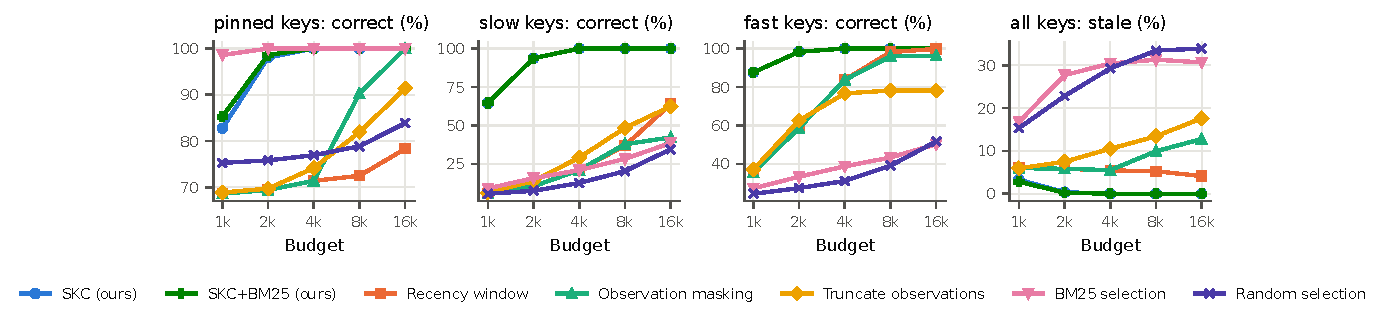
\includegraphics[width=\linewidth]{figures/synth_budget.pdf}
\caption{\textsc{StateTrack} (30 seeds): \% correct per key family and \%
stale over all keys, as a function of the budget. SKC and SKC+BM25 overlap.}
\label{fig:synth-budget}
\end{figure}

\paragraph{Budget and key families.} \Cref{fig:synth-budget} separates the
three families. Windows and masking retain fast keys once the budget covers a
few steps but lose most slow keys (at most 38\% up to 8k; window 64\% and
masking 42\% at 16k), as \cref{prop:window} predicts for small $\lambda_k$. Selection methods retain
pinned keys (their text overlaps the query) but are stale on about 30\% of all
probes from 4k up. SKC reaches 96\% correct at 2k and 100\% from 4k, with
almost no stale state. Note one subtle failure of \emph{every} baseline:
pinning the task is itself not supersession-consistent, because a user's later
revision of a pinned constraint is lost while the original stays pinned; this
accounts for the 4--6\% stale rate of the recency window.

\paragraph{Horizon.} At a fixed 4k budget (\cref{fig:synth-horizon}) the
accuracy of all baselines falls as trajectories grow from 50 to 800 steps
(window: 53\%$\to$31\%) while their stale rates grow (BM25: 24\%$\to$48\%;
window: 3\%$\to$17\%, from pinned constraints whose revisions fall out of
the window);
SKC stays at 100\%, as \cref{prop:sufficiency} predicts when the number of keys
is fixed.

\begin{figure}[t]
\centering
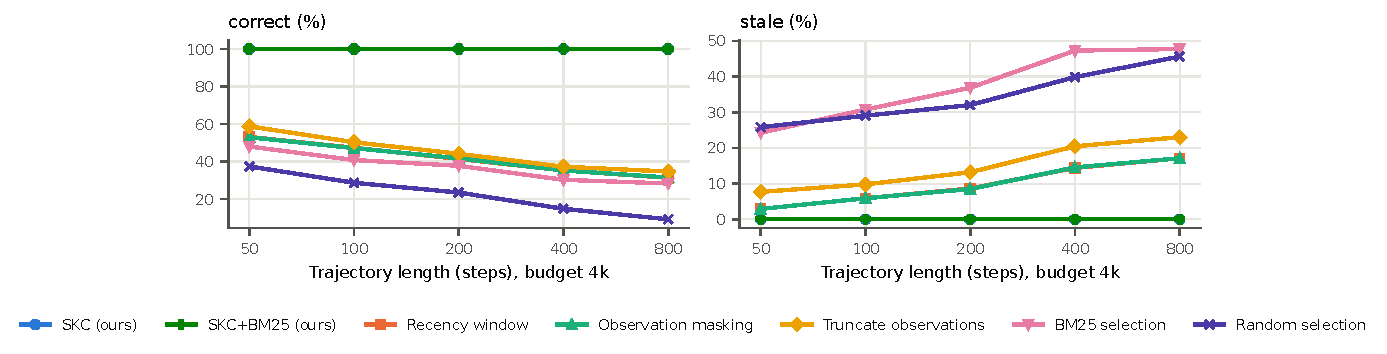
\includegraphics[width=\linewidth]{figures/synth_horizon.pdf}
\caption{\textsc{StateTrack}, budget 4k: accuracy and staleness vs.\
trajectory length. SKC and SKC+BM25 overlap at 100\% correct and 0\% stale.}
\label{fig:synth-horizon}
\end{figure}

\paragraph{Validating \cref{prop:stale}.} \Cref{fig:synth-stale} plots the
stale rate against the number of writes $m$ for random and BM25 selection,
with \cref{eq:stale} evaluated at the empirical fraction $\rho$ of turns kept.
The prediction tracks random selection closely at all three budgets; BM25 is
noisier and tends to sit above it at small budgets, because its scores are
correlated with lexical overlap rather than independent. Window and SKC are
never stale.

\begin{figure}[t]
\centering
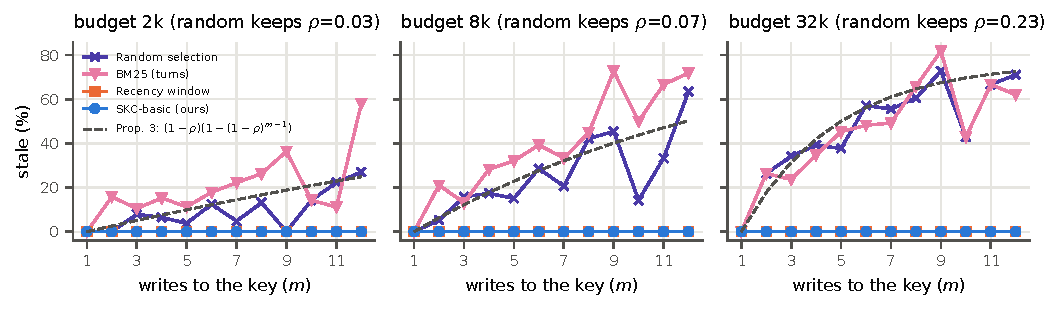
\includegraphics[width=\linewidth]{figures/synth_stale_theory.pdf}
\caption{Stale rate vs.\ number of writes per key ($m$) in \textsc{StateTrack}
(200 steps, 12 fast keys). Dashed: \cref{prop:stale} with the measured $\rho$.}
\label{fig:synth-stale}
\end{figure}

\paragraph{Imperfect extraction.} \Cref{fig:synth-recall} degrades the
extractor's recall $r$. A ledger alone (no raw window) behaves exactly as
\cref{prop:stale} predicts with $\rho=r$: at $r=0.7$, 25\% of probes are stale.
SKC's raw recent window and backward extension hedge against missed writes,
because the latest write of an actively changing key is usually recent: at 8k
and $r=0.7$, SKC is stale on 8\% of probes and correct on 88\%, against 25\% and
69\% for the ledger alone. SKC+BM25 is more exposed (16\% stale), because its
extension is supersession-blind and \cref{cor:safe} only protects keys whose
latest write the ledger actually holds. Extraction quality is therefore the
critical dependency of state-keyed methods, and when it is uncertain, the
leftover budget is better spent on a raw window than on relevance.

\begin{figure}[t]
\centering
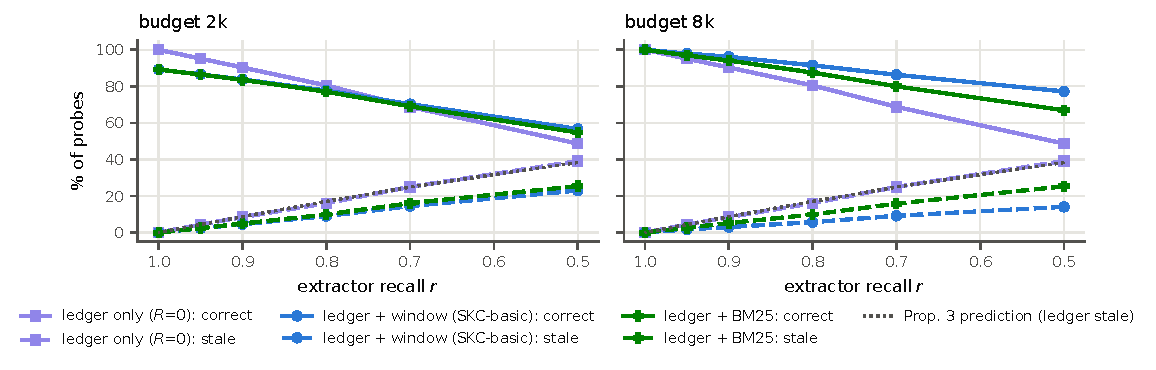
\includegraphics[width=\linewidth]{figures/synth_recall.pdf}
\caption{SKC variants under extractor recall $r$ (\textsc{StateTrack}, 30
seeds). Solid: correct; dashed: stale; dotted: \cref{prop:stale} with $\rho=r$
for the ledger alone.}
\label{fig:synth-recall}
\end{figure}

\paragraph{Capacity.} When the number of keys grows at a fixed 2k budget
(\cref{fig:synth-capacity}), SKC degrades as the ledger stops fitting (98\% at
20 keys, 64\% at 100, 28\% at 400), as the lower bound of
\cref{prop:sufficiency} requires; windows and masking fall from 29\% to 4\%.
With uniform probe probabilities and equal record sizes, every priority order
is equally good (\cref{prop:knapsack}); we verified that recency-only and FIFO
priorities match the default to within one point.

\begin{figure}[t]
\centering
\begin{minipage}{0.4\linewidth}
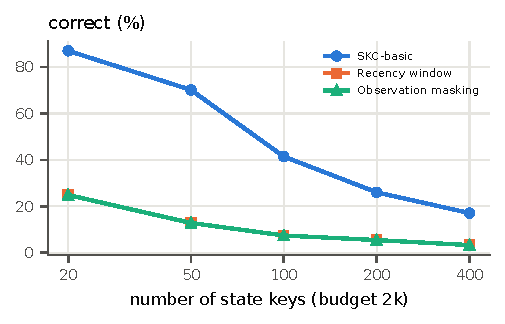
\includegraphics[width=\linewidth]{figures/synth_capacity.pdf}
\end{minipage}\hfill
\begin{minipage}{0.56\linewidth}
\caption{Retention as the number of state keys grows at a fixed 2k budget
(\textsc{StateTrack}, 200 steps). Full retention requires space linear in the
number of live keys (\cref{prop:sufficiency}); SKC degrades gracefully once the
ledger no longer fits, while windows retain only recently written keys.}
\label{fig:synth-capacity}
\end{minipage}
\end{figure}

\subsection{Ablations on real trajectories}
\label{sec:ablation}

Ablation results pending.


%% ---------------------------------------------------------------------------
\section{Discussion and Limitations}
\label{sec:limitations}

\paragraph{Sufficiency is not success.} We measure whether information is
\emph{present} for an ideal reader. Real models may fail to use information that
is present (e.g.\ in the middle of a long context~\citep{liu2024lost}) and may
recover information that is absent (by re-running a command or re-opening a
file). Our numbers are therefore upper bounds on what compression permits, not
predictions of solve rates. Measuring end-to-end task success with LLM agents
on compressed contexts is the most important next step; this study could not
call LLMs.

\paragraph{No LLM summarization baseline.} Summarization is a widely used
compressor~\citep{wang2023recursively,lindenbauer2025complexity,kang2025acon}
that we could not run. Our analysis still applies to it: a summary is
supersession-consistent only if the summarizer reliably replaces old values by
new ones, which is precisely the extraction problem of \cref{sec:synthetic},
and recursive summaries can compound such errors over time.
\citet{lindenbauer2025complexity} found that observation masking matches LLM
summarization in solve rate on SWE-bench, which suggests summarization does not
dominate the baselines we include.

\paragraph{Probe design.} State keys are derived by the same structural parser
that SKC uses, which advantages SKC on state probes. We mitigate this in three
ways: key-free use probes, a synthetic benchmark with exact ground truth, and
noisy-extractor experiments; we also report where SKC loses (file views; long
range use probes against BM25). The evidence threshold ($\theta=0.8$), the
evidence sampling, and the regular-expression token counts are design choices;
other choices change absolute numbers but not the qualitative ordering we
observed during development.

\paragraph{Domain.} Our real data come from one agent scaffold (two
generations of SWE-agent) on one task family (repository-level bug fixing).
Structural extraction is easiest when tools are typed; agents whose state
lives mostly in free text (dialogue, web browsing) need learned extractors,
whose recall then governs staleness (\cref{prop:stale}).

%% ---------------------------------------------------------------------------
\section{Conclusion}

Agent histories are event logs, and the information an agent must keep is the
current state those events define. Viewing compression through this lens
separates two failure modes---missing and stale state---and explains when
common compressors exhibit them: windows forget by age, and
supersession-blind selection retains outdated values at a rate that grows with
the number of overwrites. Log compaction is the natural remedy. A simple,
model-free implementation, SKC, retains 66--83\% of agent state on real SWE-agent
trajectories at 4k--16k tokens (vs.\ 39--66\% for windows and observation
masking) with a stale rate of 0.1\%, and its hybrid with relevance selection
also preserves the long-range information agents go on to use. The
remaining challenges are extraction for unstructured state and end-to-end
validation with LLM agents.


\bibliographystyle{plainnat}
\bibliography{refs}

\clearpage
\appendix
%% ---------------------------------------------------------------------------
\section{Proofs}
\sloppy
\label{app:proofs}

\paragraph{\Cref{prop:sufficiency}.} By construction $\mathrm{L}_t$ contains,
for every written key, the record of its latest write and no other record for
that key, so $R^\ast$ returns the value of that write, which is $S_t(k)$ by
definition. Each key contributes exactly one record whose size depends only on
the key name and its current value, so $|\mathrm{L}_t|$ is a function of
$(\mathcal{K}_t, S_t)$ alone. For the lower bound, fix $K$ keys and consider the
$|\mathcal{V}|^K$ histories that write each key once with an arbitrary value.
If two such histories with different state vectors were mapped to the same
context, $R^\ast$ would give the same answer on both for every key and hence be
wrong on at least one probe of one of them. The compressor is therefore
injective on these histories, so some context has description length at least
$\log_2|\mathcal{V}|^K = K\log_2|\mathcal{V}|$ bits. \qed

\paragraph{\Cref{prop:sc}.} Suppose an SC context has some write to $k$
present. The present writes of $k$ form a non-empty suffix of its write
sequence, which contains the latest write, so $R^\ast$ returns the latest value
(correct). Otherwise no write is present (missing). A window of whole turns
keeps a suffix of turns, hence a suffix of every key's writes. The compacted log
keeps exactly the last write of each key (a suffix of length one). If $c_1,c_2$
are SC, the present writes of $k$ in $c_1\cup c_2$ are a union of two suffixes,
which is a suffix. \qed

\paragraph{\Cref{prop:window}.} The window contains exactly the turns whose
starting position lies within the last $W$ tokens, so the latest write to $k$
is present iff it lies in that range; older writes are then absent too (no
stale outcome), and if the latest write is outside the range so are all older
ones (missing). For a stationary Poisson process with rate $\lambda_k$ per step,
the time since the last event (the age $A$) is exponentially distributed with
rate $\lambda_k$. Approximating the token distance by $\mu A$,
$\Pr[\mu A\le W]=1-e^{-\lambda_k W/\mu}$. \qed

\paragraph{\Cref{prop:stale}.} Let the writes of $k$ be in turns
$i_1<\dots<i_m$, each kept independently with probability $\rho$. The probe is
correct iff turn $i_m$ is kept ($\rho$). It is missing iff none is kept
($(1-\rho)^m$). It is stale iff $i_m$ is dropped and at least one of the $m-1$
earlier turns is kept: $(1-\rho)(1-(1-\rho)^{m-1})$ (we assume distinct
values; equal values only turn stale outcomes into correct ones). This is
increasing in $m$ with limit $1-\rho$. Conditioned on some write being present,
the stale fraction is $(1-\rho)(1-(1-\rho)^{m-1})/(1-(1-\rho)^m)\to 1-\rho$.
For an extractor with independent recall $r$ feeding a latest-wins ledger, the
ledger record of $k$ is the latest \emph{detected} write; it equals the true
latest write with probability $r$, is an older write with probability
$(1-r)(1-(1-r)^{m-1})$, and is absent otherwise, which is \cref{eq:stale} with
$\rho=r$. \qed

\paragraph{\Cref{cor:safe}.} If $k$'s record is in $\mathrm{L}'$, the latest
write of $k$ is present, so $R^\ast$ answers correctly whatever else $c'$
contains, since every other present write of $k$ is older. \qed

\paragraph{\Cref{prop:dedup}.} A line is removed from a turn only if the same
(normalized) line occurs in a later turn, the task, or the recent window, and the
latest occurrence of every line is never removed (processing turns from newest
to oldest, a line is removed only once it has been seen), so the set of distinct
lines of the history is unchanged. Turns carrying the current value of some key
are not modified, so the evidence group of every current value is identical with
and without content compaction, and a probe whose current value is present under
a selection remains present under the same selection. Removed runs are replaced
by one marker each. \qed

\paragraph{\Cref{prop:knapsack}.} The expected number of correct probes is
$\sum_k p_k\,\mathbb{1}[k\text{ kept}]$ subject to $\sum_k |\mathrm{rec}(k)|\,
\mathbb{1}[k\text{ kept}]\le B$, a 0/1 knapsack. The ratio-greedy solution of
the fractional relaxation is optimal~\citep{dantzig1957knapsack}; the better of
the greedy integral prefix and the single most valuable item achieves at least
half of the fractional optimum. \qed

%% ---------------------------------------------------------------------------
\section{Probe and Evidence Details}
\label{app:probes}

\paragraph{Evidence lines.} Values are split into lines; each line is
normalized by removing carriage returns and editor line-number prefixes
(e.g.\ \texttt{123:} or \texttt{\phantom{0}123\textbackslash t}) and collapsing
whitespace; lines shorter than 6 characters or without alphanumerics are
discarded, and duplicates are removed. For command outputs the evidence is the
last 12 such lines (results, tracebacks and test summaries are printed last);
for all other keys it is 12 lines sampled evenly across the value. A write is
present if one unit contains at least 80\% of its evidence lines. Matching is
line-exact after normalization, so an edit is also present if the file view
echoed after the edit shows the new lines.

\paragraph{Key derivation for SWE-agent.} SWE-agent 0.x actions
(\texttt{open}, \texttt{goto}, \texttt{scroll\_up}/\texttt{scroll\_down},
\texttt{create}, \texttt{edit~a:b}, \texttt{search\_dir},
\texttt{search\_file}, \texttt{find\_file}) and SWE-agent 1.x actions
(\texttt{str\_replace\_editor} with \texttt{view}, \texttt{create},
\texttt{str\_replace} or \texttt{insert}; bash) are parsed
deterministically. The currently open file in 0.x is tracked from the
\texttt{[File: \dots]} header of observations. \emph{Edit regions}: a line-range
edit supersedes an earlier edit of the same file if their line ranges overlap;
a \texttt{str\_replace} supersedes an earlier edit if its \texttt{old\_str} is
contained in, or shares an informative line with, the text written by that
edit; \texttt{create} resets the file. \emph{View windows} are bucketed by
starting line into 50-line blocks. Commands are normalized by stripping
leading \texttt{cd \dots\ \&\&} prefixes and collapsing whitespace. The task key
is the issue text; it is pinned by every compressor and therefore always
correct.

\paragraph{Use probes.} Identifiers are maximal matches of
\texttt{[A-Za-z\_][\textbackslash w./-]\{3,\}[\textbackslash w]} (names, dotted names, paths
without the leading slash). A use probe is an identifier that occurs in the
next action, is not a stop word (interface commands, Python keywords, common
shell tools), occurs in some earlier turn of the history, and does not occur
in the system prompt (which every compressor keeps). We bucket use probes by the
number of steps since the identifier \emph{last} occurred; ``long-range'' use
probes are those whose last occurrence is more than two steps back (i.e.\
outside the most recent turns that every compressor keeps).

\paragraph{Copy probes.} A copy probe is a normalized line of at least 12
characters of the next action that occurs as a line of an earlier non-system
turn and not in the system prompt; it is available if the line occurs in the
compressed context.

\paragraph{Decision points.} For each trajectory we take up to six evenly
spaced decision points (just before an agent turn) whose uncompressed history
(excluding the system prompt) exceeds 4k tokens; a budget $B$ is evaluated on
the points whose history exceeds $B$. Every compressor is evaluated on the same
points. Tokens are counted with a BPE tokenizer (the legacy Claude tokenizer
shipped with version 0.28.0 of the MIT-licensed \texttt{anthropic} Python SDK);
the system prompt, which every method keeps, is not charged to the budget.

%% ---------------------------------------------------------------------------
\section{Baseline and SKC Settings}
\label{app:settings}

\begin{itemize}[leftmargin=*,itemsep=1pt,topsep=2pt]
\item \textbf{Recency window}: task pinned; most recent whole turns that fit;
the last turn is truncated (head and tail) if it alone exceeds the budget.
\item \textbf{Observation masking}~\citep{lindenbauer2025complexity}: all agent
turns kept; tool outputs other than the 10 most recent replaced by a
placeholder; then recency window.
\item \textbf{Truncate observations}: tool outputs other than the 2 most recent
are cut to 200 tokens (one third head, two thirds tail); then recency window.
\item \textbf{BM25 selection}: last 2 turns kept; other turns ranked by BM25
($k_1=1.2,b=0.75$) against the task and the latest agent turn and added
greedily; original order preserved.
\item \textbf{Random selection}: last 2 turns kept; other turns added in random
order while they fit.
\item \textbf{BM25 chunks}: the same 12-line chunks of older turns as SKC (no
ledger, no deduplication), admitted greedily by BM25 score per token against the
task and the latest agent turn; last 2 turns kept.
\item \textbf{Self-information}: a model-free version of Selective
Context~\citep{li2023selective}: lines of older turns are ranked by their mean
self-information under a unigram model of the history and kept greedily; last
4 turns kept.
\item \textbf{SKC-basic}: ledger with priority $p_k=w_{\mathrm{type}}\tau/(\tau+\mathrm{age}_k)$
($w_{\text{edit}}=4$, $w_{\text{cmd}}=2$, $w_{\text{search}}=1.5$,
$w_{\text{view}}=1$, $\tau=20$ steps), value cap 300 tokens, $R=4$ recent turns,
remaining budget spent extending the raw window backwards and then on agent
turns only.
\item \textbf{SKC}: $R=2$, chunks of at most 12 lines / 200 tokens, value cap
$V=300$, $\lambda=0.3$, supersession-aware deduplication (lines of at least 6
normalized characters). Utility model: \texttt{HistGradientBoostingClassifier}
(300 iterations, learning rate 0.08, 31 leaves, L2 1.0), trained on up to 8
decision points per training trajectory with negatives subsampled at 30\% and
re-weighted. Features: the 28 listed in \cref{sec:method} plus three added after
a first evaluation and validated on the development split (BM25 against the
latest agent turn alone, and the number of the item's lines that also occur in
the latest agent and tool turns or in the last four turns). $R$, chunk size and
$\lambda$ were chosen on the development instances from
$\{2,4\}\times\{12,24,48\}\times\{0.1,0.3\}$ (\cref{sec:setup}). A variant
trained to predict the \emph{number} of needed pieces per item (Poisson loss),
which matches the knapsack objective more closely, was not better (within one
point on every metric) and is not used.
\end{itemize}
In \textsc{StateTrack} the extractor reads the \texttt{key = value} lines that
carry writes; on SWE-agent it is the structural parser above. Noisy extractors
drop each write independently (deterministically by a hash of key and turn)
with probability $1-r$.

%% ---------------------------------------------------------------------------
\section{Additional Results}
\label{app:results}

\begin{table}[h]
\centering
\small
\caption{Real trajectories at 8k, per model. Top: \% of state probes correct.
Bottom: \% of long-range use probes (last seen $>$2 steps earlier) available.}
\label{tab:by-model}
\setlength{\tabcolsep}{5pt}
\begin{tabular}{l rrrrr}
\toprule
Compressor & GPT-4 & Claude 3 Opus & GPT-4o & Claude 3.7 S. & Claude 4 S. \\
\midrule
\multicolumn{6}{l}{\emph{State probes: correct (\%)}} \\
Recency window        & 61.4 & 76.9 & 54.8 & 59.4 & 41.9 \\
Observation masking   & 59.7 & 72.6 & 51.6 & 45.8 & 30.8 \\
Truncate observations & 61.7 & 74.6 & 58.8 & 51.6 & 45.7 \\
BM25 selection        & 63.1 & 77.7 & 60.5 & 51.7 & 31.6 \\
Random selection      & 75.6 & \textbf{91.6} & 73.3 & 65.3 & 52.9 \\
SKC (ours)            & \textbf{77.0} & 90.0 & 81.5 & 76.2 & 73.0 \\
SKC+BM25 (ours)       & 75.2 & 89.4 & \textbf{83.0} & \textbf{77.1} & \textbf{73.3} \\
\midrule
\multicolumn{6}{l}{\emph{Use probes, long range: available (\%)}} \\
Recency window        & 81.1 & 87.9 & 70.0 & 84.5 & 82.5 \\
Observation masking   & 82.4 & 89.5 & 71.9 & 78.8 & 83.8 \\
Truncate observations & \textbf{93.7} & 85.5 & 86.0 & 79.6 & 87.5 \\
BM25 selection        & 91.2 & 94.4 & 79.8 & 91.6 & \textbf{89.1} \\
Random selection      & 92.9 & \textbf{96.0} & \textbf{95.6} & 86.0 & 82.7 \\
SKC (ours)            & 93.3 & 93.5 & 94.6 & 85.6 & 80.8 \\
SKC+BM25 (ours)       & 91.6 & 93.5 & 89.7 & \textbf{92.1} & 85.1 \\
\bottomrule
\end{tabular}
\end{table}

The per-model breakdown shows that the advantage of SKC on state probes grows
with trajectory length: it is smallest for Claude~3 Opus (median 18 steps,
where random selection of a short history already covers most of it) and
largest for Claude~4 Sonnet (median 59 steps). On long-range use probes no
method dominates across models; SKC+BM25 is best or within 4 points of the best
for four of the five models.


\end{document}
